\chapter{Biblioteca bempp.}\label{sec:Biblioteca bempp.}
\setcounter{figure}{0}
\setcounter{equation}{0}
Bempp es una plataforma computacional gratuita de elementos de frontera se puede utilizar para resolver problemas de acústica o electroestática, entre otros. Utiliza una interfaz de python de fácil uso, en nuestro caso utilizamos $Docker$\footnote{Software que crea contenedores virtuales para que puedan ejecutarse bajo cualquier máquina, independiente del sistema operativo que tenga.} $Images$ para poder resolver nuestro problema.\\ 
Como se vio en la sección anterior, para resolver problemas con BEM es necesario resolver sistemas compuestos por matrices de gran tamaño, las cuales a su vez contienen elementos que son necesario aproximar, es por esto que la existencia de esta libreria abierta facilita la tarea.
\section{Estructura.}
La librería bempp tiene una estructura basada en la imagen \ref{fig:Estructura BEM}, la cual tiene 5 grandes ejes y es explicado con mayor detalle en \cite{Solvingwithbempp}:
\begin{itemize}
\item Grid: Responsable del manejo de la malla, apoyado en la librería 'Dune-FoamGrid'.
\item Fiber (\textbf{F}ast \textbf{I}ntegration \textbf{B}oundary \textbf{E}lement \textbf{R}outine): Es un elemento vital dentro de la librería. Encargado de evaluaciones las integrales de elementos de borde en cada elemento, sin importar su conectividad. Además de realizar la integración como tal. Este modulo es independiente del resto por lo que podría ser utilizado de manera particular en otros códigos de BEM.
\item Space: Responsable del espacio de funciones y sus derivadas. También actúa como administrador de grados de libertad, usando los conocimientos de la conectividad entre elementos y las propiedades de continuidad del espacio de funciones.
\begin{figure}[H]
\centering
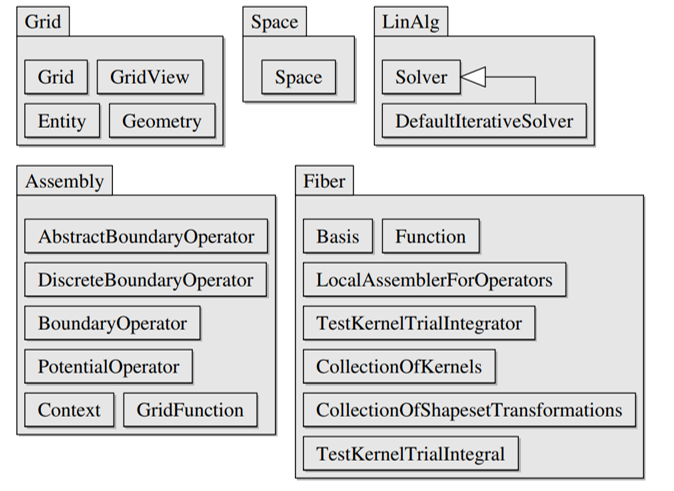
\includegraphics[scale=0.7]{Imagenes/estructurabempp.png}
\caption{Modulos de bempp (Fuente:\cite{Solvingwithbempp})}\label{fig:Estructura BEM}
\end{figure}
\item Assembly: Es el modulo más grande de la librería. Define los operadores integrales y los espaciones de funciones en la malla. También almacena las matrices de las integrales discretizadas que son formadas en el módulo Fiber.
\item LinAlg: Módulo que almacena distintos tipos de $solver$'s lineales. 
\end{itemize} 


\subsection{Algoritmo y explicación.}
Antes de comenzar a desmenuzar la resolución del problema o el código utilizado es más importante definir que es \textbf{bempp}\cite{bempp}.\\
 El algoritmo para la resolución de problemas a través de bempp es más bien simple pero es necesario tener los conceptos claros o no podremos ejecutarlo de forma correcta. La forma de resolución es la que se muestra a continuación. Es necesario indicar que esta resolución resolvera los parametros de borde, para resolver los elementos internos simplemente se debe realizar una nueva malla con puntos internos y utilizar la solución calculada.
 \begin{figure}[H]
 \centering
 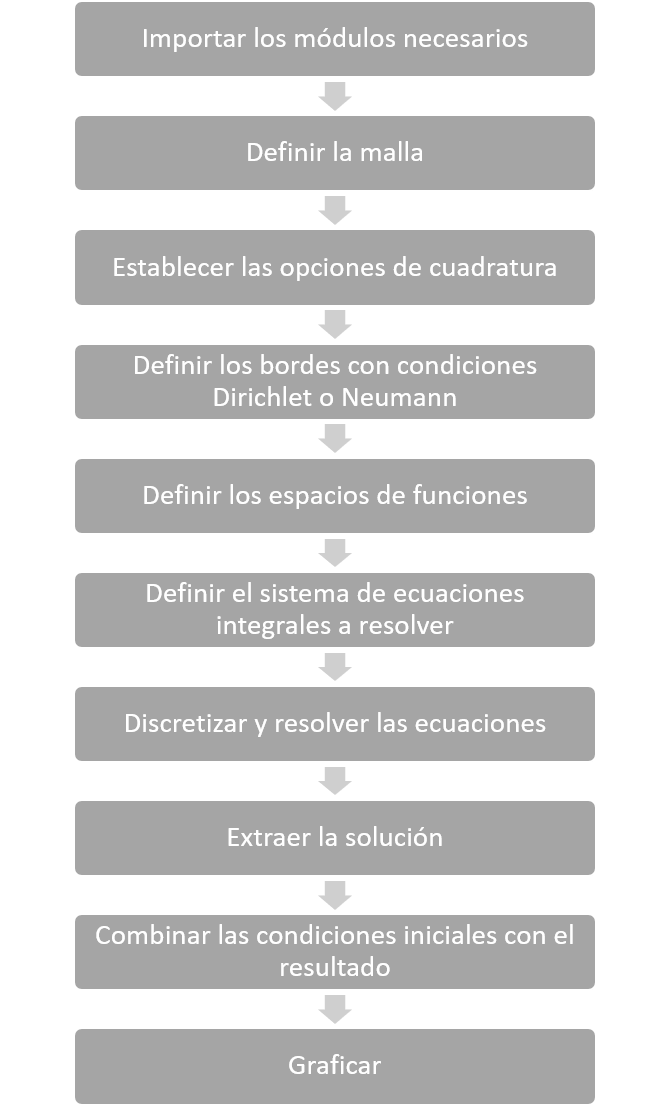
\includegraphics[scale=0.75]{Imagenes/Algoritmo bempp.png}
 \caption{Algoritmo resolución bempp}\label{fig:Algoritmo de BEM}
 \end{figure}

Al observar el esquema se nos hace evidente definir los conceptos y además mostrar como se ejecutó lo descrito en el código:
\begin{enumerate}
\item \textbf{Importar los módulos necesarios.}\\
Módulos: También conocidas como bibliotecas o librerías, añaden funciones adicionales a nuestro lenguaje de programación de uso: Python. Para resolver el problema se utilizaron 3: numpy, scipy.sparse.linalg (para resolver sistemas lineales) y por supuesto, bempp.
\item \textbf{Definir la malla.}\\Malla - Grid: El mallado en esta plataforma puede realizarse de manera bastante simple, siempre y cuando la figura sea común (esferas, cubos, etc...). Estas también pueden ser importadas desde el formato Gmsh.
\item \textbf{Establecer las opciones de cuadratura.}\\Cuadratura - Quadrature: Como vimos en el código manual, hay que utilizar una cuadratura Gaussiana para resolver las ecuaciones integrales, en este punto se precisa de cuantos puntos se hará esa cuadratura. Para asimilar esta forma de resolución lo más posible a la anterior utilizaremos nuevamente 4 puntos.
\item \textbf{Definir los espacios de funciones.}\\Conocido como espacio de función o Function spaces. Como sabemos los nodos podían ser tomados para medios constantes, lineales o polinomiales, dependiendo del medio en que queramos definir nuestros nodos, nuestros espacios de función deben ser definidos en el orden deseado. En la plataforma bempp es importante definir esto correctamente. Como se señala en el algortimo es necesario haber generado con anterioridad la malla, ya que esto es un input necesario. Los tipos de 'Function spaces' que nos interesan son escalares y son utilizados para resolver problemas de Laplace y Helmholtz:
\begin{itemize}
\item \textbf{Continuos Polynomial "P": } Se refiera a que el 'espacio' entre nodos debe tener continuidad, a modo de ejemplo se tiene la figura \ref{fig:Interseccion elementos continuos} la cual nos muestra una intersección de elementos lineales continuos. Este espacio no puede utilizarse con elementos constantes ya que todos deberían ser la misma constante lo cual carece de sentido, es por esto que el orden de este espacio va desde 1 (lineal) hasta 10.
\item \textbf{Discontinuos Polynomial "DP": }Caso contrario al anterior, en donde la intersección de los elementos no necesariamente debe tener una continuidad, es por esto que cuando se desea tener elementos constantes es necesario utilizar este tipo de espacio. El rango del orden va desde 0 (constante) hasta 10.
\item \textbf{Dual spaces "DUAL": }Este tipo de espacio está disponible solo para orden 0. Estos	 espacios forman un emparejamiento dual estable junto con funciones lineales continuas a trozos y son necesarios para ciertos precondicionadores de orden opuesto
\end{itemize}

\begin{figure}[H]
\centering
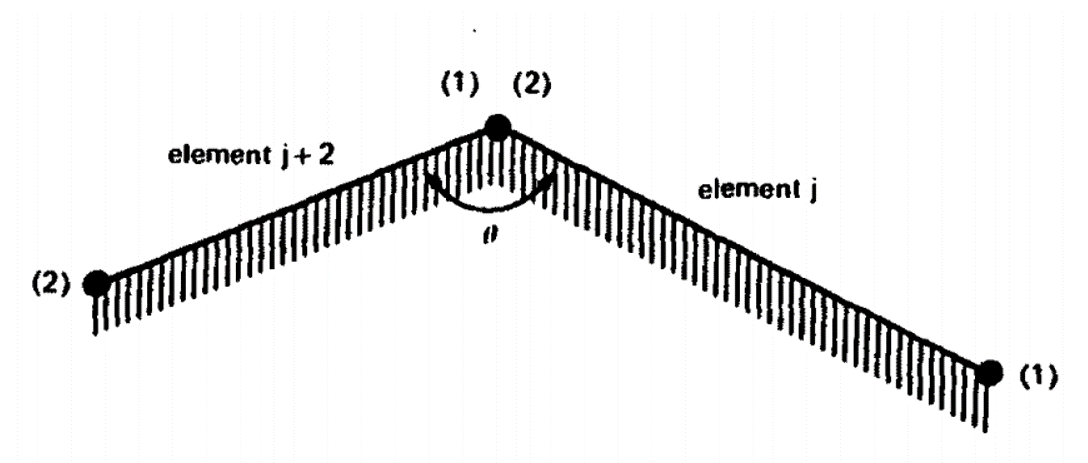
\includegraphics[scale=0.4]{Imagenes/nodos lineales continuos.png}
\caption{Intersección de elementos lineales continuos (Fuente:\cite{Brebbia})}\label{fig:Interseccion elementos continuos}
\end{figure}
\item \textbf{Definir el sistema de ecuaciones integrales a resolver.}\\
Operadores - Operators: Lo que en la ecuación \eqref{eq:Descripcion de matriz H y G} describimos como matrices $H$ y $G$, en esta plataforma son conocidos como operadores ('Single Layer Operator' y 'Double Layer Operator' respectivamente) y no son los únicos que están disponibles. Se definen de la siguiente forma:
\begin{equation}
\label{eq:Operadores de Laplace}
\begin{split}
V=\int_\Gamma g(x,y)d\Gamma\qquad & \textnormal{Single Layer Operator} \\
K=\int_\Gamma \frac{\delta g(x,y)}{\delta y}d\Gamma\qquad & \textnormal{Double Layer Operator} \\
K'=\int_\Gamma \frac{\delta g(x,y)}{\delta x}d\Gamma\qquad & \textnormal{Adjoint Double Layer Operator} \\
H=-\frac{\delta}{\delta x}\int_\Gamma \frac{\delta g(x,y)}{\delta y}d\Gamma\qquad & \textnormal{Hypersingular Boundary Operator} 
\end{split}
\end{equation}
Es importante destacar que es necesario precisar el modulo en el que serán ocupados: Laplace, Helmholtz o Helmholtz modificado. Existen otro operadores importantes como el operador de matriz identidad. La función $g(x,y)$ es la función de Green, la cual en todo este informe hemos definido como $u$.\\  
{Funciones de malla - Grid function: }Se trata de la función dominante, la función potencial en la frontera del elemento de estudio. También se utiliza para definir la condiciones de frontera de nuestro problema. En nuestro caso, las Grid function utilizadas fueron las condiciones de Neumann y Dirichlet indicadas en el problema.        
{Generación y resolución del sistema lineal: }Una vez que se tiene definido todo lo anterior se procede a definir el lado izquiero y derecho de la ecuación del problema, el cual posteriormente será resuelto usando $gmres$ al igual que el código anterior.
\item \textbf{Discretizar y resolver las ecuaciones.}\\
Ahora que ya calculamos el potencial y su derivada en los bordes es hora de calcular el comportamiento en su interior. Para eso haremos una matriz de vectores y 'anclaremos' en un punto en el eje $z$ para poder mostrar los resultados en un gráfico 2D al igual que en el código de Brebbia y Dominguez facilitando así la comparación de resultados.
Por útlimo se calculan los potenciales con las soluciones que obtuvimos en la parte anterior y se grafican.
\end{enumerate}